\chapter{Introduction}
\label{chap:introduction}
\setcounter{page}{1}
\pagenumbering{arabic}
The general objective of computer vision-based analysis of surveillance video in busy public scenes has achieved increasing attention in the last decade, both because of tremendous potential practical application value such as security monitoring and academy research challenges.
Video event recognition is a crucial application of video understanding. 
It aims to automatically detect and report situations of special interest, in particular when abnormal events happen.
Most of the existing solutions work in well-constrained surveillance settings and show good results if they are tuned to a specific predefined application. 
Many of them focus on recognition of basic human actions~\cite{zhou2009human, marszalek2009actions} (like ''walking'', ''jumping''), simple activities~\cite{wang2014hierarchical} or interactions among a few agents (normally two)~\cite{sun2013active}.
However, the scenarios in real world monitored scenes are much more complicated, especially in public busy scenes, e.g., a crowded traffic scene, a busy train station or a shopping mall (see~Fig.~\ref{fig:example_scenes}). Video events in these scenes are complex, ambiguous and not well defined. 
%Ideally, a system would autonomously learn model of the scene to interpret the scene and automatically recognize abnormal events. 

\begin{figure}[!htbp]
	\centering
	\subfigure[Traffic junction]{
		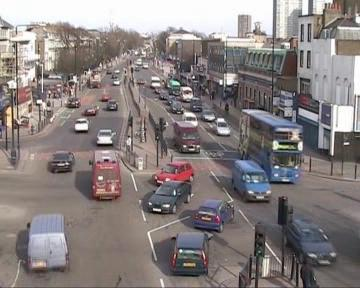
\includegraphics[width = 3.6cm, height = 2.5cm]{figures/traffic_scene.jpg}
	}
	\subfigure[Shopping mall~\cite{shoppingmallimg}]{
		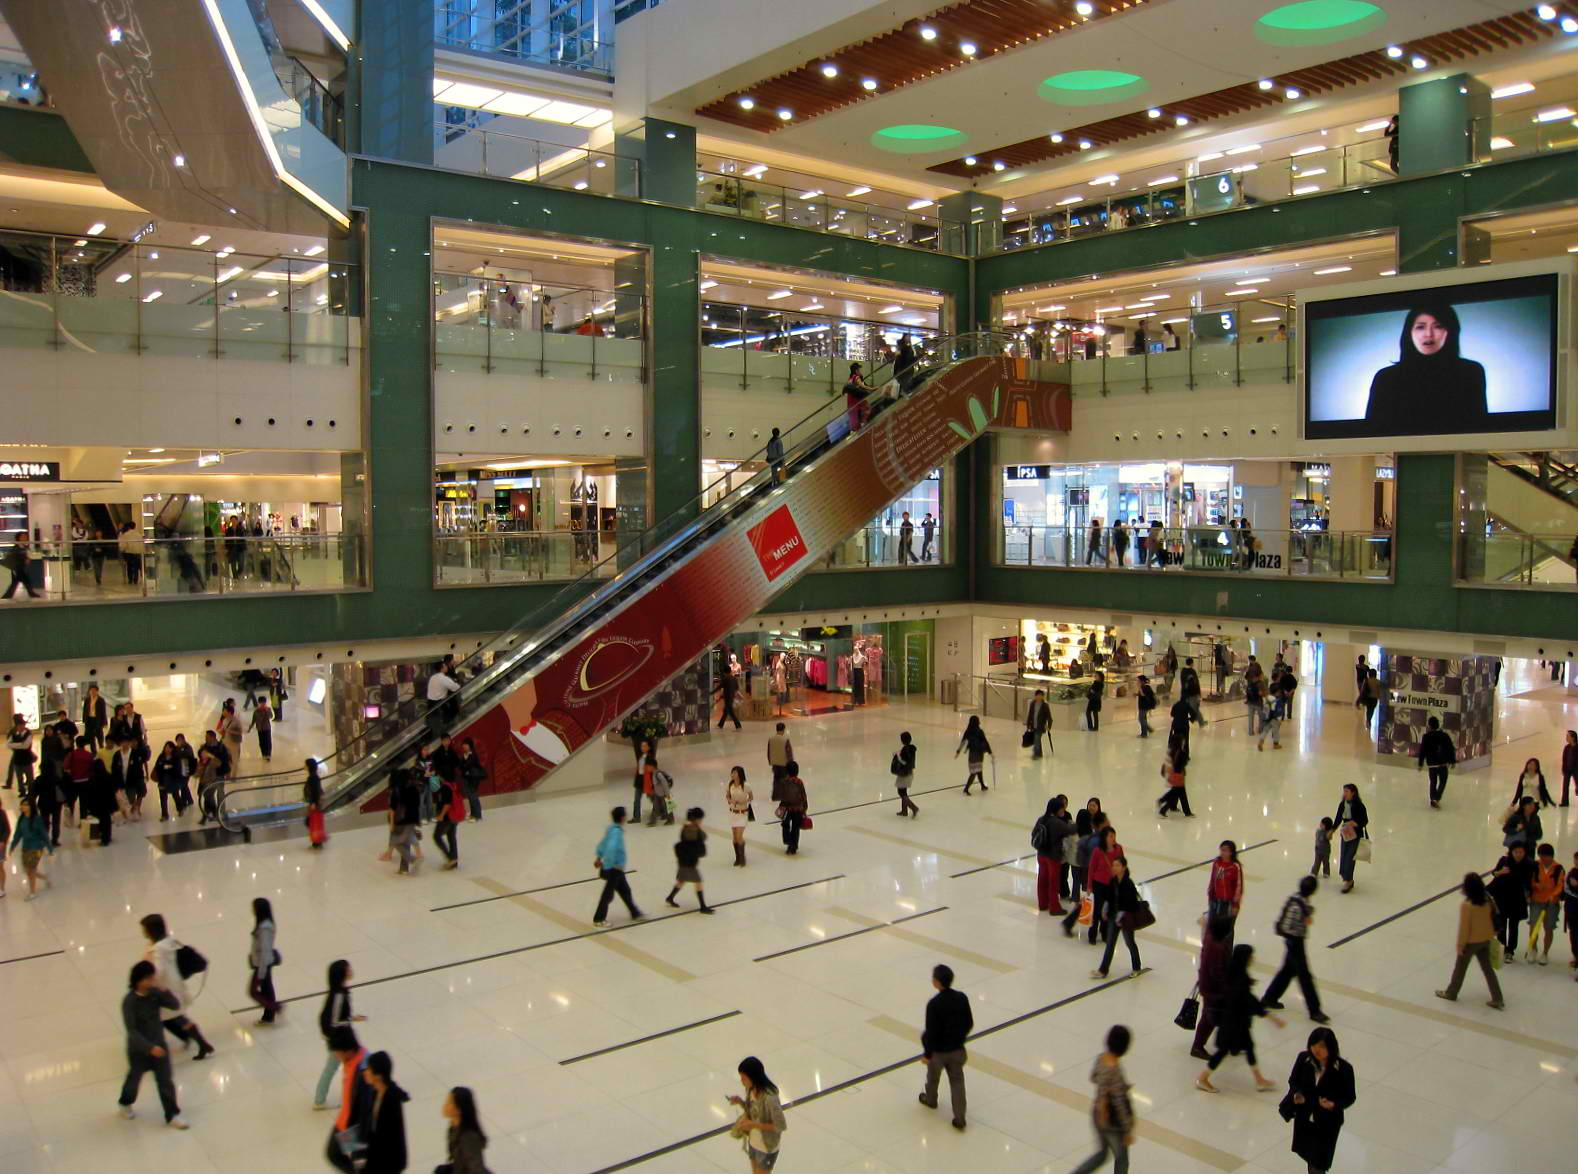
\includegraphics[width = 3.6cm, height = 2.5cm]{figures/crowded-shopping.jpg}
	}
	\subfigure[Subway station~\cite{subwayimage}]{
		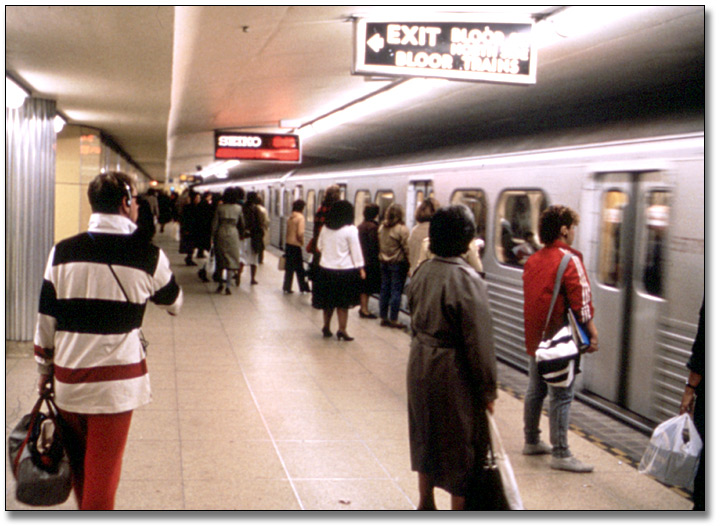
\includegraphics[width = 3.6cm, height = 2.5cm]{figures/subway_station.jpg}
	}
	\subfigure[Train station~\cite{trainimage}]{
		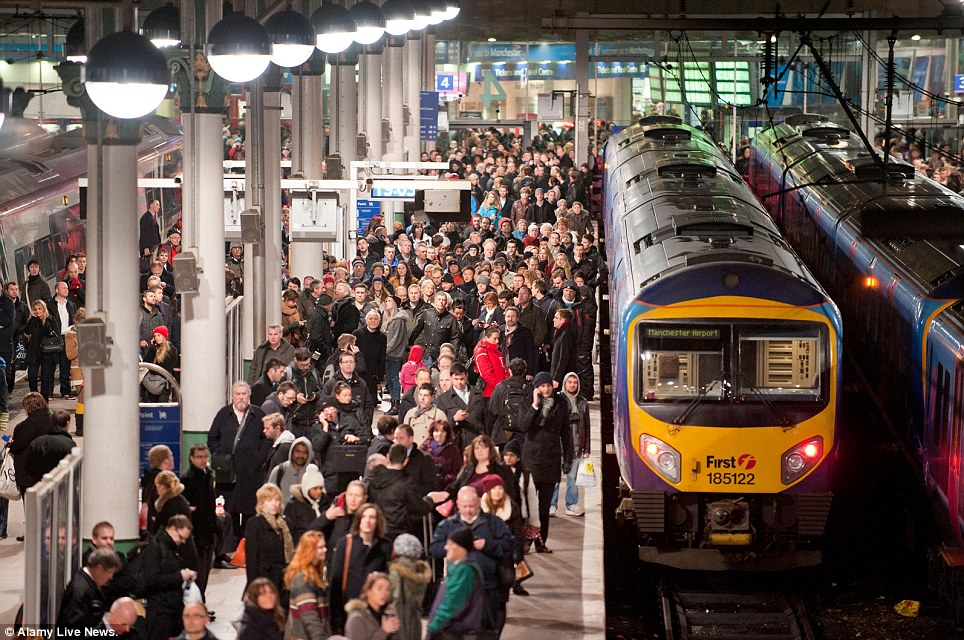
\includegraphics[width = 3.6cm, height = 2.5cm ]{figures/train_station.jpg}
	}
	\caption[Examples of crowded and complicated public scene]
	{Examples of crowded and complicated public scene.}
	\label{fig:example_scenes}
\end{figure}

\begin{figure}[!htbp]
	\centering
	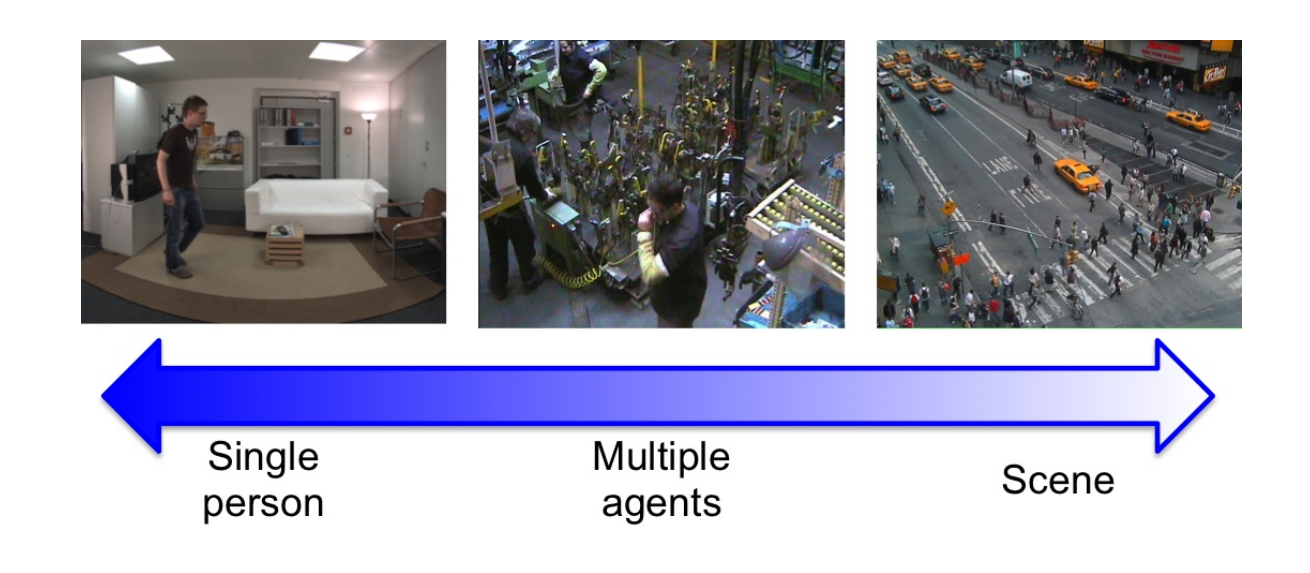
\includegraphics[width = 1 \textwidth]{figures/event_level.jpg}
	\caption[Different visual surveillance scenarios at varying scale levels]
	{ Different visual surveillance scenarios at varying scale levels. They are defined as low-level, middle-level and high-level events respectively~\cite{nater2012abnormal}.}
	\label{fig:event_level}
\end{figure}

To analyze the scenarios in these complicated and crowded scenes, recent research in video event recognition has shifted to classifying complex events which contain many activities and agents~\cite{swears2014complex, kinoshita2014traffic, wang2009unsupervised}. Such complex events are usually called as interactions, or more professionally as high-level events when compared with the low-level basic human action and middle-level activities. The hierarchical relationship is illustrated in Fig.~\ref{fig:event_level}. The goal of high-level video event recognition is to automatically identify video clips that contain events of interest. A high-level event can be reasonably defined as a combination of different types of co-occurring atomic activities. For instance, a car stops at a crossroad to wait for the other cars that have the right of way.

%********************************************************************************************
\section{Motivation}
\label{motivation}
The number of surveillance cameras installed to monitor private and public spaces keeps increasing dramatically since the last decade. 
This is mainly due to the rising demand for commercial or security interest in public scenes. However, the online video streams from surveillance cameras are watched by trained human operators (see Fig.~\ref{fig:manual_watch}) traditionally. 
This method is expensive, laborious, low efficient and really unreliable.
Ideally, users would like the ability to automatically analyze the surveillance video for robustly reporting the situations and identifying abnormal events in real-time.
Therefore, the visual surveillance market has urgent and high demands for adequate algorithms or software solutions, which would automatically analyze the scene, recognize video events, detect anomalies and alarm the operators.

\begin{figure}[!htbp]
	\centering
	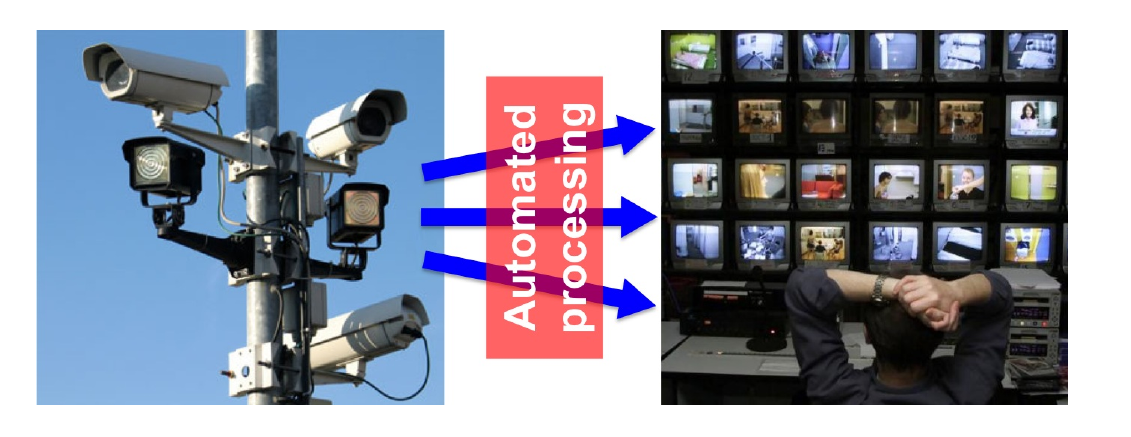
\includegraphics[width = 0.8 \textwidth]{figures/human_watched.jpg}
	\caption[Surveillance video are watched by human operators]
	{Traditional and most commonly nowadays approach to analyze surveillance video is manually~\cite{nater2012abnormal}.}
	\label{fig:manual_watch}
\end{figure}

The main challenges for this task in crowded public scenes are summarized follows: 
\begin{itemize}
	\item[1] There is a large number of agents of interest. It is hard to detect or track an individual agent, especially in a far field scene where the objects of interest such as people are too small to be exactly detected.
	\item[2] There are variety of potentially interesting behaviors. They often happen simultaneously and frequently.
	\item[3] Normally, an activity is hard to be well defined in a busy public space. 
	\item[4] Abnormal events are often visually subtle compared to more obvious ongoing behaviors. They are often ambiguous between normal and abnormal. Furthermore, some abnormal events rarely happen. We have few examples to learn from and define them.
	\item[5] The surveillance videos captured by fixed cameras from a crowded scene are generally low-quality: noise, low resolution, etc.
	\item[6] Robustness and computational tractability are the most challenging problems for an approach to work well in real-time.
\end{itemize}

Much study has focused on either applying supervised learning methods \cite{altun2004gaussian, robertson2006general} or unsupervised density estimation methods \cite{wang2009unsupervised, li2008global}. The former methods learn discriminative models to classify behaviors and identify anomalies. They have the advantage in terms of classification accuracy. However, supervised methods require a large number of examples for different classes of behaviors to learn from. The manual effort required to label training data could be prohibitively expensive. Moreover, examples of rare behaviors are hard to be collected. The latter methods learn generative models of normal behavior and can thereby potentially identify abnormal events as outliers. However, this kind of methods is often computation consuming. After learning, they do not enjoy comparable accuracy as the discriminative models for classification. Furthermore, their online working modes are time and computation consuming due to the computation of joint distribution.

Motivated by the advantages and limitations of these two models, we address to combine their advantages together to construct a novel framework. It would automatically learn the typical activities and interactions by means of the generative models from  video datasets which are captured by static cameras form complicated and crowded traffic scenes. The learning results would exercise the discriminant models. Then, the trained classifier would classify interactions and identify abnormal events in the online captured video from the same spots.


%******************************************************************************
\section{Contribution}
\label{contribution}


In this thesis, we provide an efficient unsupervised learning framework for automatically analyzing surveillance videos of crowed and complicated traffic scenes, modeling the activities and interactions, classifying the interactions and detecting abnormal events in real-time. 
The main contributions in this paper are summarized as follows: 
\begin{itemize}
	\item We effectively combine unsupervised generative model HDP with supervised discriminant model GP, to realize unsupervised classification of video event.
	\item To construct suitable feature vectors for supervised GP classifier, we provide a method to represent the atomic activities using low-level visual features and to represent the interactions using typical atomic activities.
	\item The temporal dependencies between two interactions are integrated into GP classifier to enhance the accuracy of the classification.
	\item We provide detailed experiments and analysis showing that our framework enjoys favorable performance in video event classification in real-time in crowded and complicated traffic scenes. Three benchmark datasets: QMUL Junction Dataset, QMUL Junction Dataset 2~\cite{hospedales2009markov} and MIT Dataset~\cite{wang2009unsupervised}.
\end{itemize}

To our best knowledge, our study is the first attempt to combine non-parametric generative HDP model and discriminant GP model for unsupervised online video events recognition and anomalies detection in a complicated and crowded traffic scene.
%******************************************************************************
\section{Organization of the Thesis}
\label{outline}
This thesis is structured as follows:

In Chapter~\ref{chap:relatedwork}, we will discuss about the related works. Some of the most popular researches and techniques are introduced. Additionally, the advantages and limitations of the approaches will also be demonstrated.

Chapter~\ref{chap:bg} will introduce the theories about the generative probability topic models and discriminative model Gaussian process for regression and classification which will be adopted in our framework.

In Chapter~\ref{chap:framework}, we will discuss our proposed framework in detail.

Chapter~\ref{chap:experiment} presents the experimental results and provides detailed analysis. We evaluate our proposed framework on three standard video datasets over crowded traffic scenes. 

Chapter~\ref{chap:conclusion} finally concludes this thesis, discusses the important findings
and gives lines of future research. 
